\begin{frame}{Simulation of discrete system}
  Two methods have been used to simulate the discrete system.
  \begin{tabular}{l l}
  	\begin{minipage}{0.5\textwidth}
  		\begin{block}{Deterministic methode}
		\begin{itemize}
		\item Uses the Markov framework
		\item Transition matrix
		\item Fast
		\item Easy to implement
		\item No direct physics involved, just mathematics
		\item Can be speed up by linearisation
		\end{itemize}
  		\end{block}
  	\end{minipage}
  	\begin{minipage}{0.5\textwidth}
  			\begin{block}{ Stochastic methode}
  				\begin{itemize}
  				  \item Uses the a jump process
  				  \item The outcome is random
  				  \item One jump at the time
  				  \item Slow
  				  \item Represents the physical system very good
  				  \item Can produce more stochastic information
  				\end{itemize}
  		  	\end{block}
  	\end{minipage}
  	\end{tabular}
\end{frame}
\begin{frame}{Deterministic method}
\vspace{-1.5cm}
    	\begin{tabular}{l l}
    	  	\begin{minipage}{0.5\textwidth}
    	  	\begin{block}{Algorithme }
    	  	     	  		\begin{itemize}
    	  	     	  		\item Create  a transition matrix  $M(T)$
    	  	     	  		\item Chose an initial distribution  $\rho_0$
    	  	     	  		\item Update the distribution  $ \rho(t) = \rho_0 e^{Mt}$
    	  	     	  		\item Calculate the energy $E$
    	  	     	  		\item Change the temperature by a small fraction
    	  	     	  		\item repeat this process
    	  	     	 \end{itemize}
    	  	\end{block}
    	  	\end{minipage}
    	  	\begin{minipage}{0.6\textwidth}
    	  			\begin{block}{}
    	  				\begin{figure}
    	  						\centering
    	  						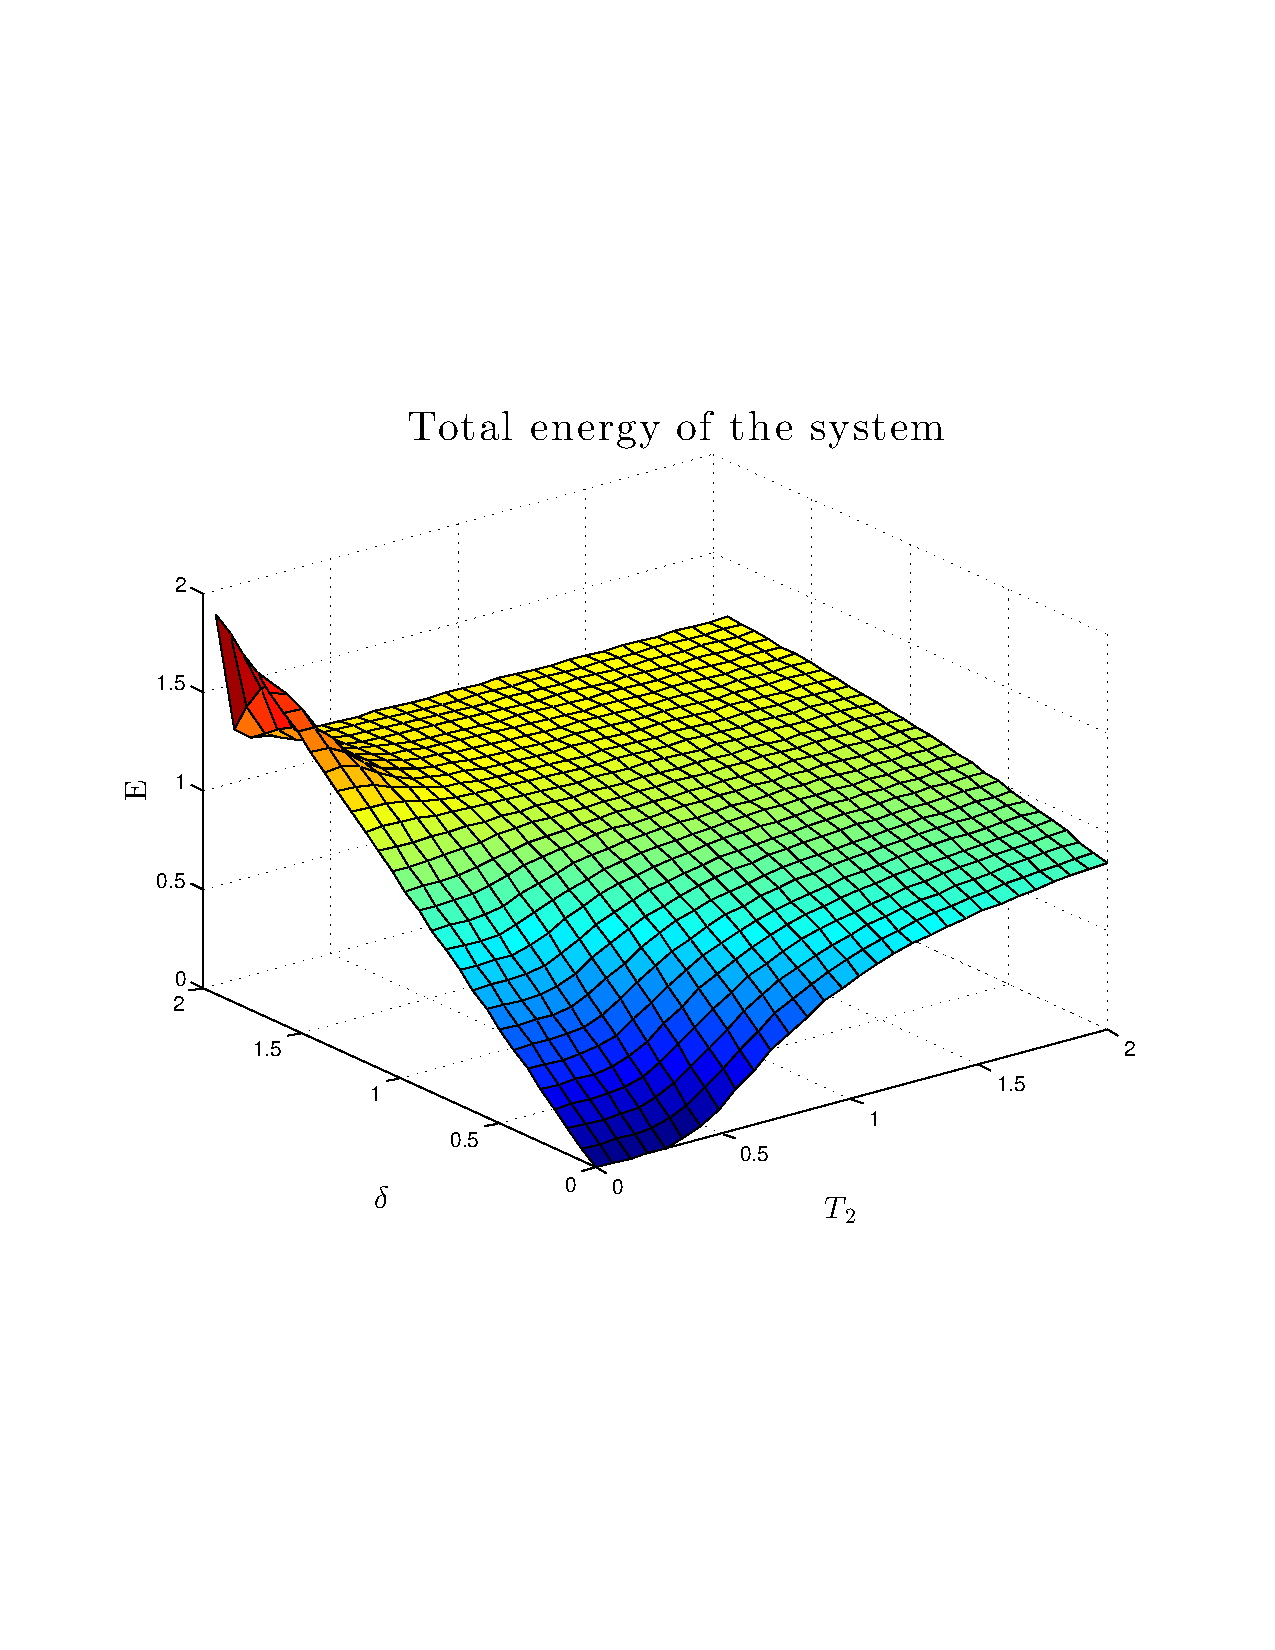
\includegraphics[width=\textwidth]{../src/plot/discreteSystems/TotalEnergyFunctionOfT2.pdf}
    	  					\end{figure}
    	  		  	\end{block}
    	  	\end{minipage}
    	  	\end{tabular}	
    	
\end{frame}

\begin{frame}{Stochastic method}
  \vspace{-1.5cm}
      	\begin{tabular}{l l}
      	  	\begin{minipage}{0.5\textwidth}
      	  	\begin{block}{Algorithme }
      	  	     	  		\begin{itemize}
      	  	     	  		\item Pick a random starting position
      	  	     	  		\item Let the particle jump for some steps
      	  	     	  		\item Calculate the energy
      	  	     	  		\item Repeat this for a good result
      	  	     	  		\item Change the temperature by a small fraction
      	  	     	  		\item repeat this process
      	  	     	 \end{itemize}
      	  	\end{block}
      	  	\end{minipage}
      	  	\begin{minipage}{0.6\textwidth}
      	  			\begin{block}{}
      	  				\begin{figure}
      	  						\centering
      	  						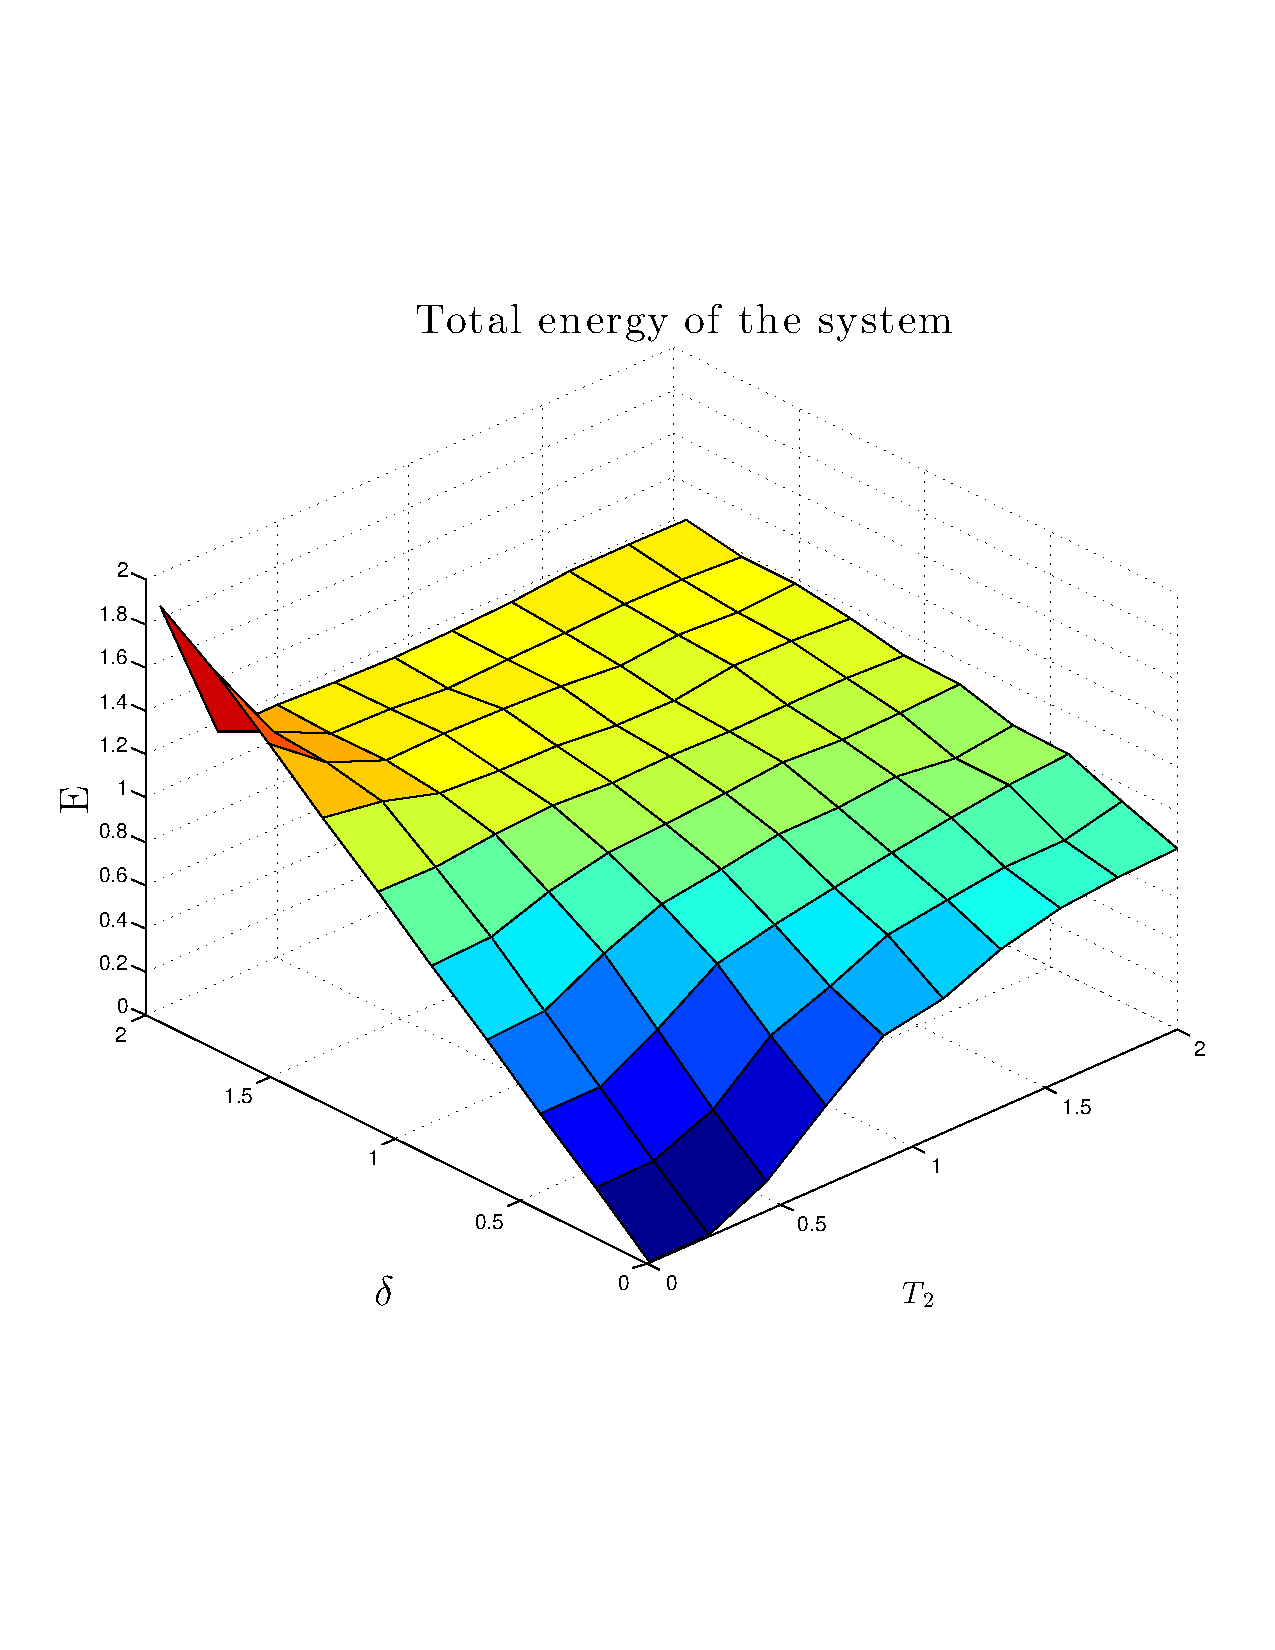
\includegraphics[width=\textwidth]{../src/plot/discreteSystems/TotalEnergyFunctionOfT2Stochastic.pdf}
      	  					\end{figure}
      	  		  	\end{block}
      	  	\end{minipage}
      	  	\end{tabular}	
      	
\end{frame}

\begin{frame}{Comparison of the two results}

     \vspace{1cm}
     
      	  	\begin{minipage}{0.49\textwidth}
      	  	\begin{block}{Two transitions }
      	  				\vspace{-1.7cm}
      	  	     	  	\begin{figure}
      	  	     	  	      	  \centering
      	  	     	  	      	  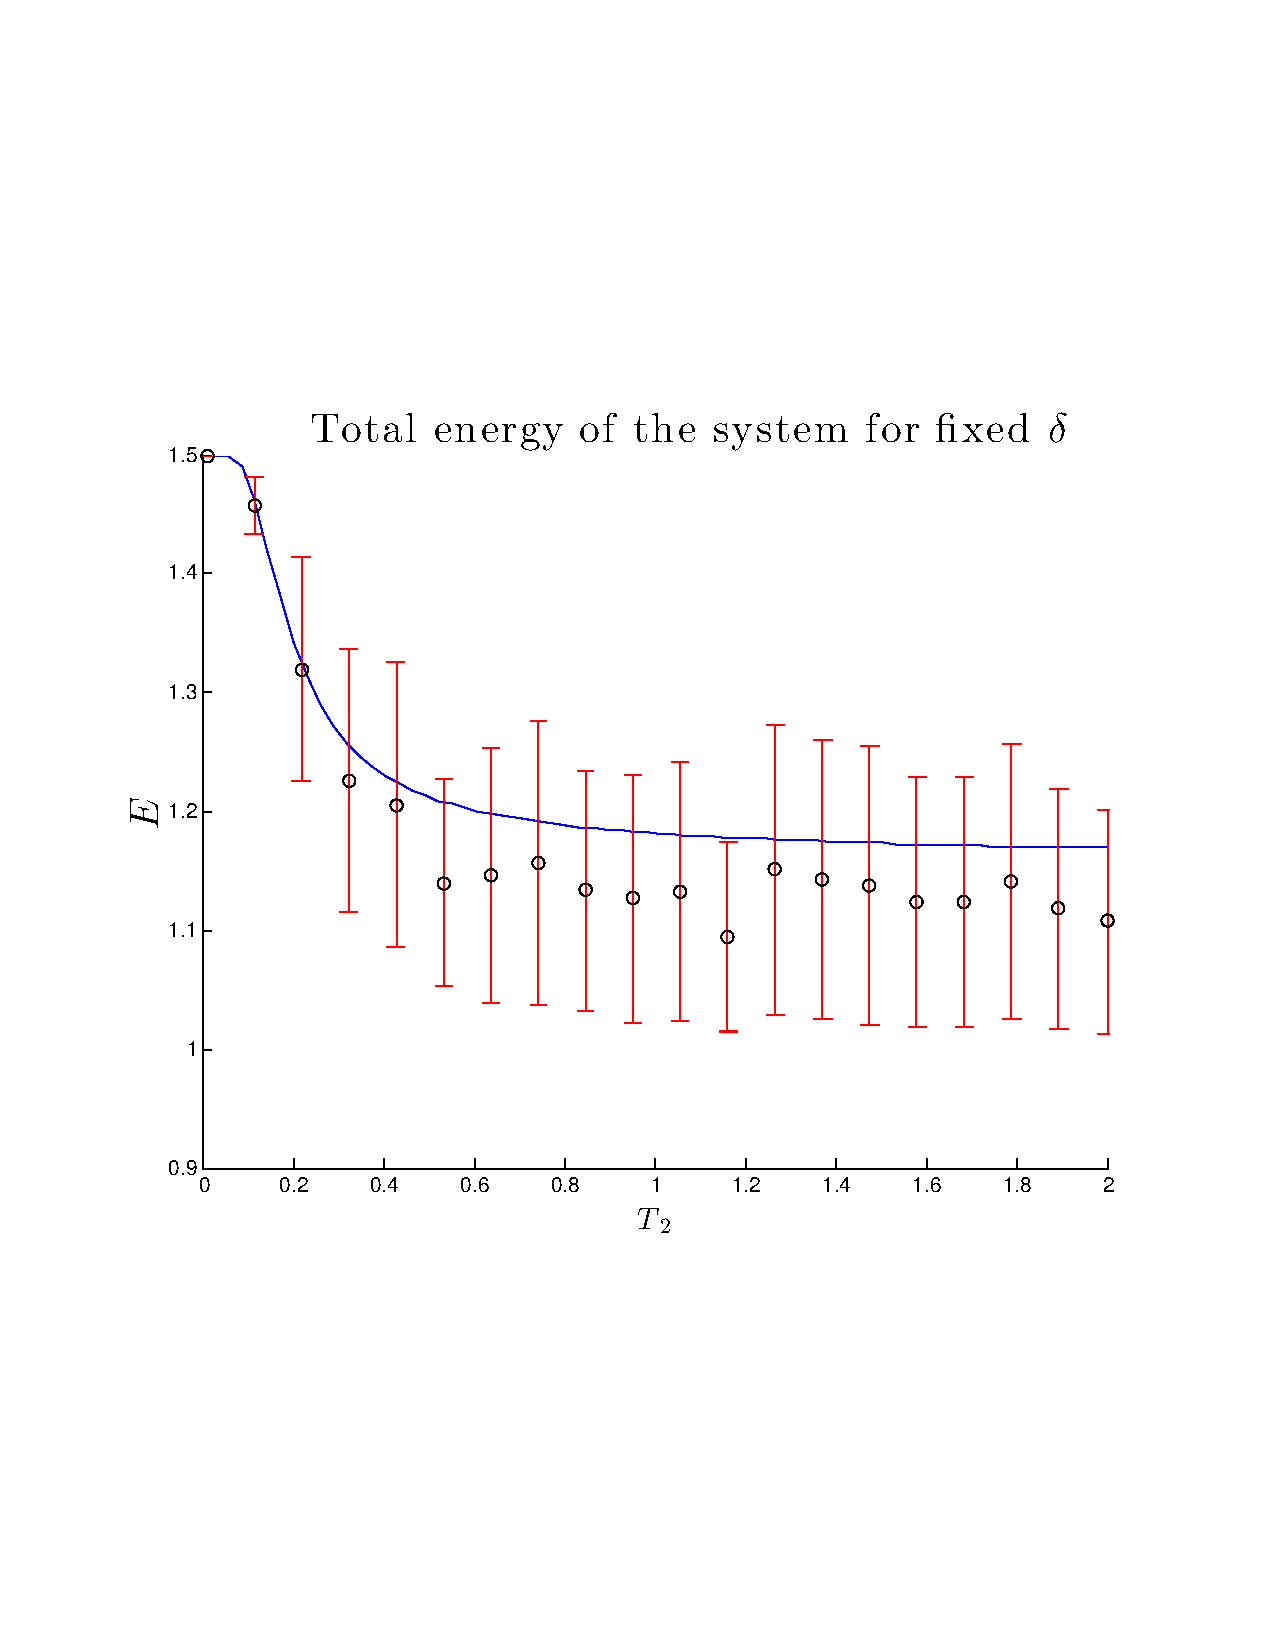
\includegraphics[width=\textwidth]{../src/plot/discreteSystems/AllInOneFixedTemp.pdf}
      	  	     	  	 \end{figure}
      	  	\end{block}
      	  	\end{minipage}
      	  	\begin{minipage}{0.49\textwidth}
      	  			\begin{block}{Three transitions}
      	  			\vspace{-1.7cm}
      	  				\begin{figure}
      	  						\centering
      	  						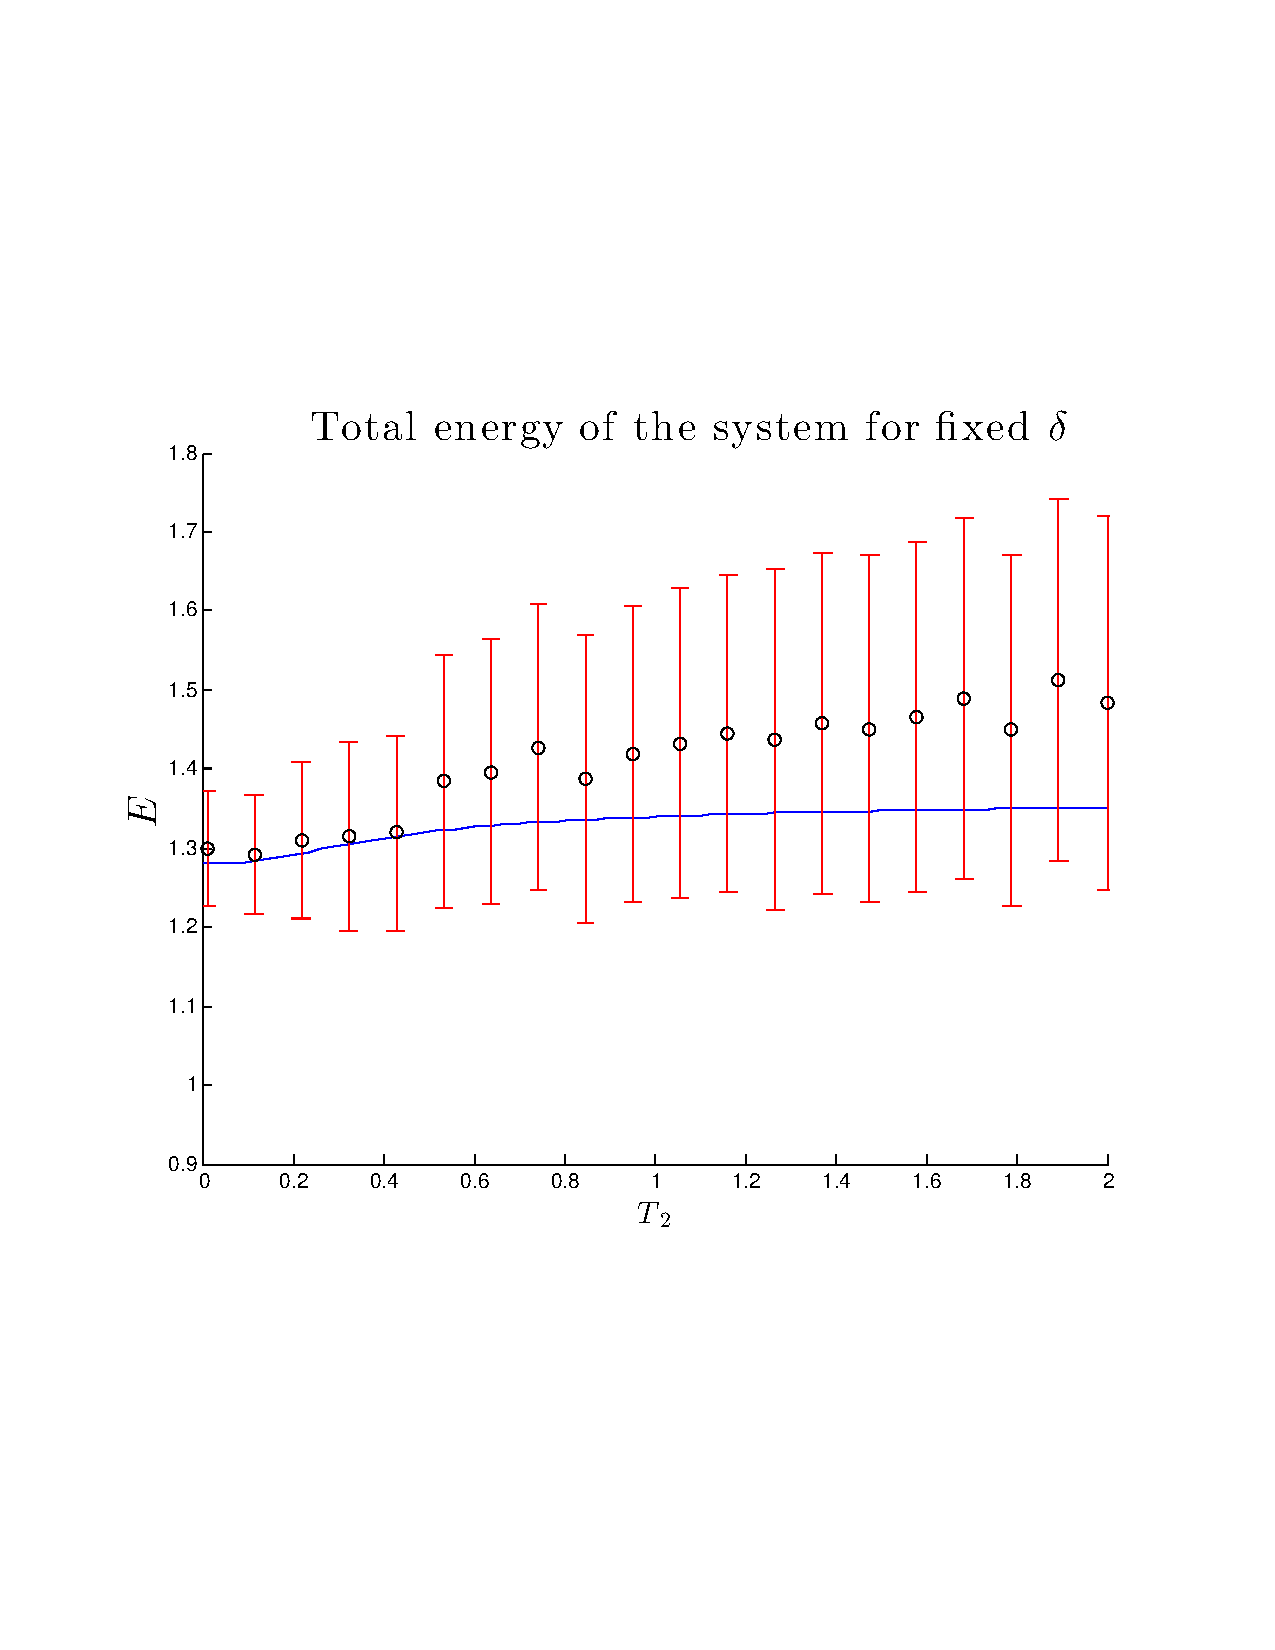
\includegraphics[width=\textwidth]{../src/plot/discreteSystems/AllInOneFixedTemp3transitions.pdf}
      	  					\end{figure}
      	  		  	\end{block}
      	  	\end{minipage}

      	
\end{frame}